\documentclass{article}[12pt]
\usepackage{amsmath}
\usepackage{amsfonts}
\usepackage{siunitx}
\usepackage{graphicx}
\usepackage{hyperref}

\sisetup{per-mode=symbol}
\hypersetup{
    colorlinks=true,
    linkcolor=blue,
    filecolor=magenta,
    urlcolor=blue
}

\title{Microelectronic Circuits Assignment 1}
\author{Sai Kartik, Manpreet Singh, Rajeev Rajagopal}
\date{February, 2022}

\begin{document}
\maketitle
\section*{Question 1}
Value of components (resistor/capacitor) present in the circuit:
\begin{table}[ht]
    \centering
    \caption{Calculated values for question 1}
    \begin{tabular}{|c | c | c|}
        \hline
        Sl. No. & Component Name & Value       \\
        \hline
        1       & R1(k$\Omega$)  & 15k$\Omega$ \\ %last digit of first group member ID+10=5+10=15
        2       & C1 (nF)        & 1nF         \\ %0.1*(last digit of 3rd group member ID+tut sec number) = 0.1*(7+3)=1
        \hline
    \end{tabular}
    \label{tab:values1}
\end{table}
\subsection*{Circuit as on LT SPICE}
%add circuit diagram
\subsection*{Graphs}
%add graphs: frequency response, input, output and transfer characteristics
\subsection*{Miscellaneous calculations}
%find DC operating point, small signal equivalent
\newpage
\section*{Question 2}
Value of components (resistors/gain) present in the circuit
\begin{table}[ht]
    \centering
    \caption{Calculated values for question 2}
    \begin{tabular}{|c | c | c|}
        \hline
        Sl. No. & Component Name   & Value               \\
        \hline
        1       & $R_1$(k$\Omega$) & 30k$\Omega$         \\ %(last digit of 3rd group member ID+3) * tut section = (7+3)*3 = 30
        2       & $R_2$(k$\Omega$) & 17k$\Omega$         \\ %product of last two digits of 1st group member ID + tut section = (3*5)+2=17
        3       & $R_3$(k$\Omega$) & 30k$\Omega$         \\ %sum of last three digits of 2nd group member ID % 8)* tut section = (4+1+9)%8*3=30
        4       & $R_4$(k$\Omega$) & 50k$\Omega$         \\ %product of last two digits of 3rd group member ID + tut section = (7+3)*3 = 30
        5       & k                & 18 \si{\volt/\volt} \\ %last 2 digits of 1st group member admission year - tut section = 20-2=18
        \hline
    \end{tabular}
    \label{tab:values2}
\end{table}
\subsection*{Circuit as on LT SPICE}
\begin{figure}[ht]
    \centering
    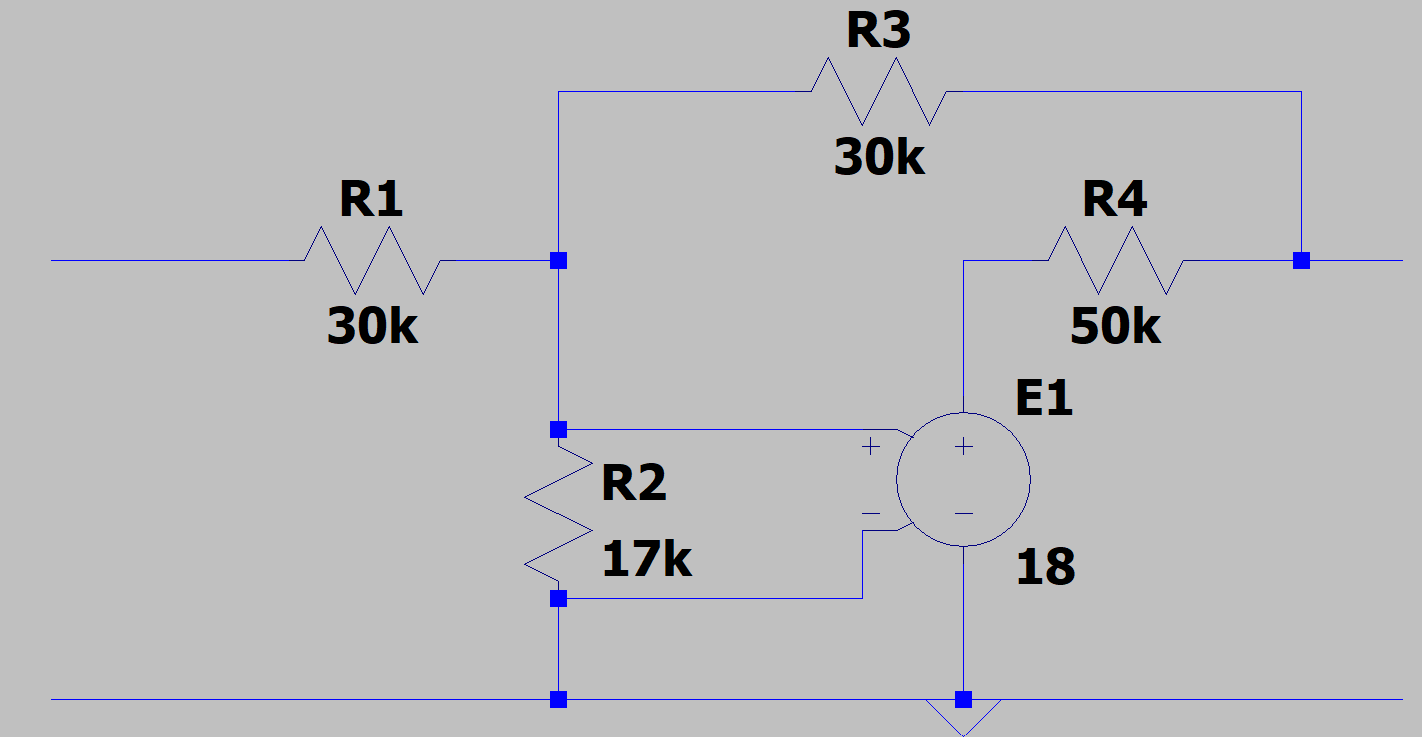
\includegraphics[scale=0.25]{orgcircuit.png}
    \caption{Original 2 port network simulated on LT SPICE}

\end{figure}
%add circuit diagram
\subsection*{Z, Y and h Parameters}
%add Z, Y and h parameters
\subsubsection*{Z parameters}
Z parameters as obtained from LT SPICE
$$ Z = \begin{bmatrix}
        23.492822k\Omega & -4.0669856k\Omega \\
        -47.99043k\Omega & -11.24402k \Omega
    \end{bmatrix}
$$
\subsubsection*{Y parameters}
$$ Y = \begin{bmatrix} %fill matrix with proper values
        0.0k\mho & 0.0k\mho \\
        0.0k\mho & 0.0k\mho
    \end{bmatrix}
$$
\subsubsection*{H parameters}
$$ H = \begin{bmatrix} %fill matrix with proper values
        0.0k\Omega & 0.0      \\
        0.0        & 0.0k\mho
    \end{bmatrix}
$$
\newpage
\subsection*{Calculations}
%add hand calculations of Z, Y and h parameters
\subsubsection*{Z parameters}
\begin{figure}[ht]
    \centering
    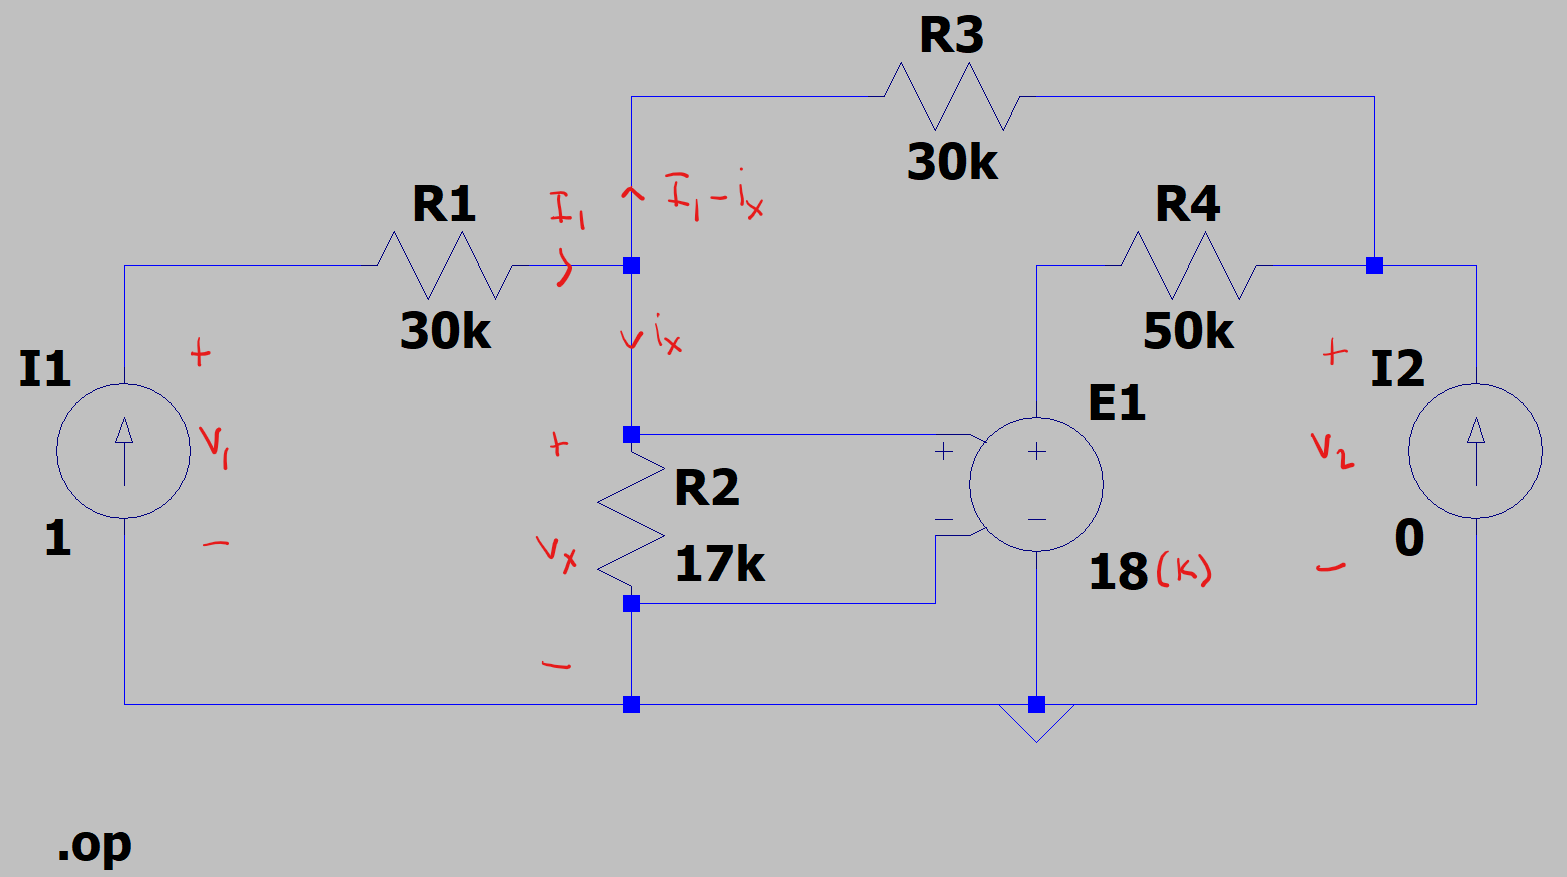
\includegraphics[scale=0.25]{zparams1.png}
    \caption{Z parameter circuit 1 (for $z_{11}$ and $z_{21}$)}
\end{figure}
Assume the convention in the above circuit for the calculations that follow
\begin{gather*}
    -(I_1-i_x)(R_3+R_4)-kV_x+V_x=0\\
    (i_x-I_1)(R_3+R_4)=V_x(k-1)\\
    (i_x-I_1)(R_3+R_4)=i_xR_2(k-1)\\
    i_x(R_3+R_4-R_2(k-1))=I_1(R_3+R_4)\\
    \implies i_x=I_1\frac{(R_3+R_4)}{R_3+R_4-R_2(k-1)} \\
    V_1=I_1R_1+V_x\\
    V_1=I_1R_1+i_xR_2\\
    V_1=I_1\left(R_1+\frac{R_2(R_3+R_4)}{R_3+R_4-R_2(k-1)}\right) \\
    \implies \frac{V_1}{I_1}=\boxed{z_{11} = R_1 + \frac{R_2(R_3+R_4)}{R_3+R_4-R_2(k-1)}} \\
    \mathrm{Also:} \\
    V_2=(I_1-i_x)R_4+kV_x\\
    V_2=(I_1-i_x)R_4+ki_xR_2\\
    V_2=i_x(kR_2-R_4)+I_1R_4\\
    V_2=I_1\left(R_4+\frac{(kR_2-R_4)(R_3+R_4)}{R_3+R_4+R_2(k-1)}\right)\\
    \implies\frac{V_2}{I_1} = \boxed{z_{21} = R_4 + \frac{(kR_2-R_4)(R_3+R_4)}{R_3+R_4-R_2(k-1)}}
\end{gather*}
\newpage
\begin{figure}[ht]
    \centering
    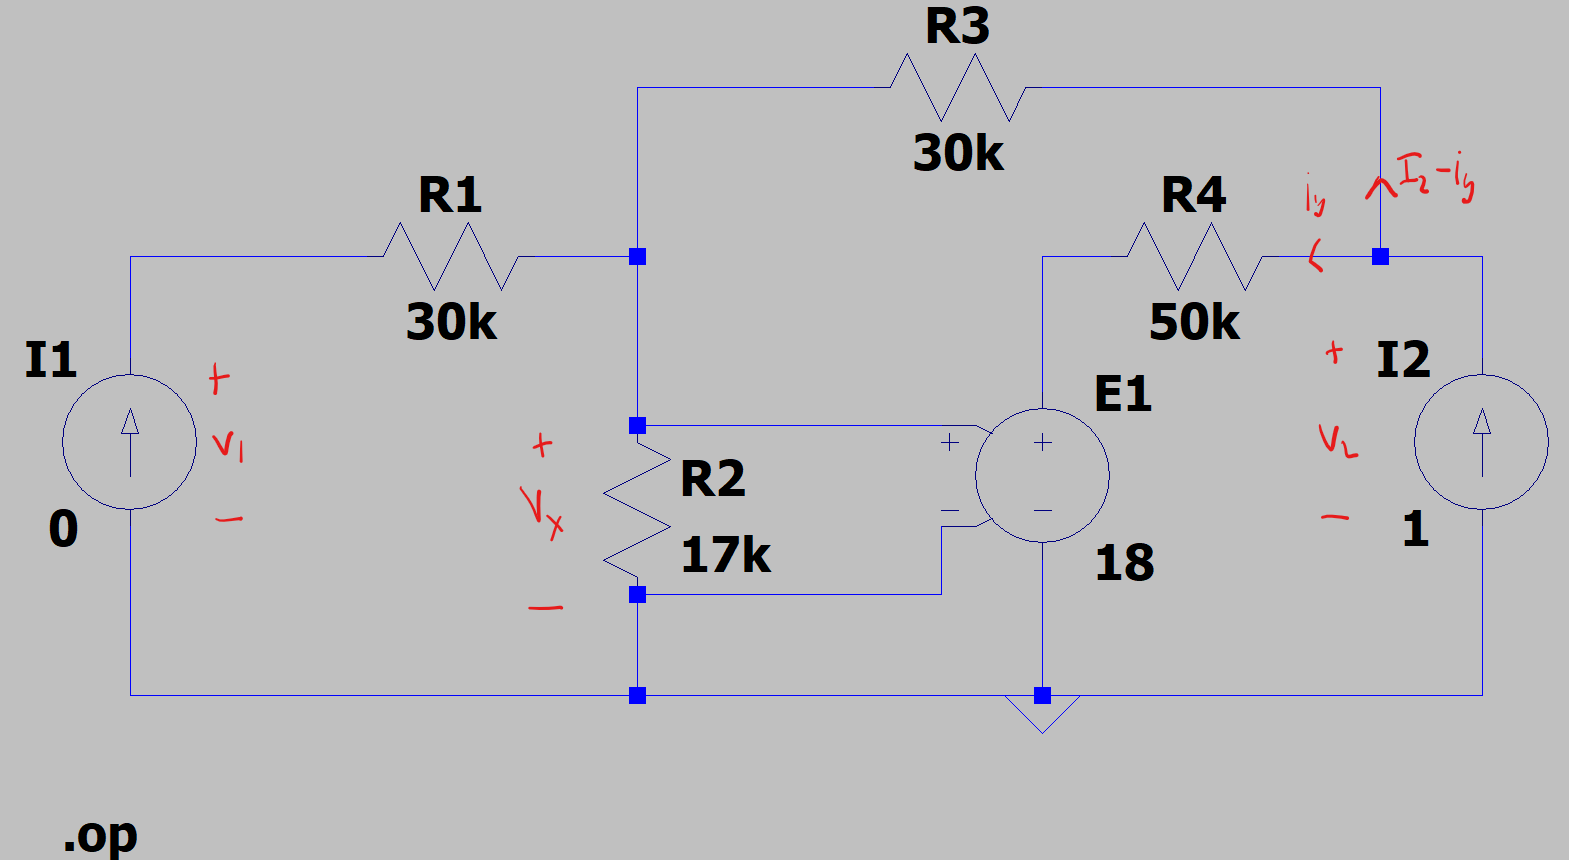
\includegraphics[scale=0.25]{zparams2.png}
    \caption{Z parameter circuit 2 (for $z_{12}$ and $z_{22}$)}
\end{figure}
Assume the convention in the above circuit for the calculations that follow
\begin{gather*}
    -R_3(I_2-i_y)-V_x+kV_x+i_yR_4=0\\
    i_yR_4-R_3(I_2-i_y)=(1-k)V_x\\
    i_yR_4-R_3(I_2-i_y)=(1-k)(I_2-i_y)R_2\\
    i_yR_4=(I_2-i_y)[(1-k)R_2+R_3]\\
    (R_4+R_3+(1-k)R_2)i_y=I_2[(1-k)R_2+R_3]\\
    \implies i_y=I_2\frac{(1-k)R_2+R_3}{(1-k)R_2+R_3+R_4}\\
    V_2=i_yR_4+kV_x\\
    V_2=i_yR_4+k(I_2-i_y)R_2\\
    V_2=i_y[R_4-kR_2]+KI_2R_2\\
    V_2=I_2\left[\frac{(R_4-kR_2)[(1-k)R_2+R_3]}{(1-k)R_2+R_3+R_4}+kR_2\right]\\
    \implies \frac{V_2}{I_2} = \boxed{z_{22} = \frac{(R_4-kR_2)[(1-k)R_2+R_3]}{(1-k)R_2+R_3+R_4}+kR_2}\\
    \mathrm{Also:} \\
    V_1=V_x=(I_2-i_y)R_2\\
    V_1=I_2R_2\left[1-\frac{(1-k)R_2+R_3}{(1-k)R_2+R_3+R_4}\right]\\
    \implies \frac{V_1}{I_2} = \boxed{z_{12} = R_2\left[1-\frac{(1-k)R_2+R_3}{(1-k)R_2+R_3+R_4}\right]}
\end{gather*}
\newpage
Using the corresponding values taken from \hyperref[tab:values2]{\ref{tab:values2}} into the above equations, we get the matrix for the Z parameters:
$$ Z = \begin{bmatrix}
        23.49282297k\Omega  & -4.066985646k\Omega  \\
        -47.99043062k\Omega & -11.244041914k\Omega
    \end{bmatrix}
$$
Which is in accordance with the values obtained from the simulation.
\subsection*{Load resistance value at port 2}
%calculate according to question given
\end{document}